\documentclass[8pt,a4paper,compress]{beamer}

\usepackage{/home/siyer/lib/slides}

\title{Minimum Spanning Trees}
\date{}
\begin{document}
\begin{frame}
\vfill
\titlepage
\end{frame}

\begin{frame}
\frametitle{Outline}
\tableofcontents
\end{frame}

\section{What are Minimum Spanning Trees?}
\begin{frame}[fragile]
\begin{itemize}
\item a spanning tree of a graph is a connected subgraph with no cycles that includes all the vertices

\item a minimum spanning tree (MST) of an edge-weighted undirected graph is a spanning tree whose weight (the sum of the weights of its edges) is no larger than the weight of any other spanning tree

\begin{center}
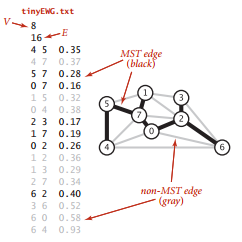
\includegraphics[scale=0.4]{./figures/mst1.png}

\smallskip

\tiny an edge-weighted graph and its MST
\end{center}

\item if the graph is connected and the edge weights are unique, then MST exists and is unique

\item goal: given a connected undirected graph $G$ with arbitrary (but distinct) edge weights, find the MST of $G$
\end{itemize}
\end{frame}

\begin{frame}[fragile]
\begin{itemize}
\item typical MST applications

\begin{center}
\begin{tabular}{ccc}
\textbf{application} & \textbf{vertex} & \textbf{edge} \\ \hline \\
circuit & component & wire \\
airline & airport & flight route \\
power distribution & power plant & transmission lines \\
image analysis & feature & proximity relationship
\end{tabular}
\end{center}
\end{itemize}
\end{frame}

\section{Edge-Weighted Graph API}
\begin{frame}[fragile]
\begin{itemize}
\item weighted-edge data type: API and implementation
\begin{lstlisting}[language={},mathescape]
public class Edge implements Comparable<Edge>

    Edge(int v, int w, double weight) // create a weighted edge $v$-$w$
    double weight()                   // edge weight
    int either()                      // either endpoint
    int other(int v)                  // the endpoint that's not $v$
\end{lstlisting}

\begin{lstlisting}[language=Java]
public class Edge implements Comparable<Edge> {
    private final int v, w;
    private final double weight;

    public Edge(int v, int w, double weight) {
        if (v < 0 || w < 0) { throw new IndexOutOfBoundsException(); }
        if (Double.isNaN(weight)) { throw new IllegalArgumentException(); }
        this.v = v; this.w = w; this.weight = weight;
    }

    public double weight() { return weight; }

    public int either() { return v; }

    public int other(int vertex) {
        if      (vertex == v) { return w; }
        else if (vertex == w) { return v; }
        else { throw new IllegalArgumentException(); }
    }

    public int compareTo(Edge that) {
        if      (this.weight() < that.weight()) { return -1; }
        else if (this.weight() > that.weight()) { return +1; }
        else                                    { return  0; }
    }
    ...
}
\end{lstlisting}
\end{itemize}
\end{frame}

\begin{frame}[fragile]
\begin{itemize}
\item edge-weighted graph (API)
\begin{lstlisting}[language={},mathescape]
public class EdgeWeightedGraph

    EdgeWeightedGraph(int V)  // create an empty graph with $V$ vertices
    EdgeWeightedGraph(In in)  // create a graph from input stream
    int V()                   // number of vertices 
    int E()                   // number of edges
    void addEdge(Edge e)      // add weighted edge e to this graph
    Iterable<Edge> adj(int v) // edges incident to $v$
    Iterable<Edge> edges()    // all edges in this graph
\end{lstlisting}
\end{itemize}
\end{frame}

\begin{frame}[fragile]
\begin{itemize}
\item edge-weighted graph: implementation
\begin{lstlisting}[language=Java]
public class EdgeWeightedGraph {
    private final int V;
    private int E;
    private LinkedBag<Edge>[] adj;
    
    public EdgeWeightedGraph(int V) {
        if (V < 0) { throw new IllegalArgumentException(); }
        this.V = V;
        this.E = 0;
        adj = (LinkedBag<Edge>[]) new LinkedBag[V];
        for (int v = 0; v < V; v++) {
            adj[v] = new LinkedBag<Edge>();
        }
    }

    public EdgeWeightedGraph(In in) {
        this(in.readInt());
        int E = in.readInt();
        if (E < 0) { throw new IllegalArgumentException(); }
        for (int i = 0; i < E; i++) {
            int v = in.readInt();
            int w = in.readInt();
            double weight = in.readDouble();
            Edge e = new Edge(v, w, weight);
            addEdge(e);
        }
    }
    
    public int V() { return V; }

    public int E() { return E; }
    ...
}
\end{lstlisting}
\end{itemize}
\end{frame}

\begin{frame}[fragile]
\begin{itemize}
\item edge-weighted graph: implementation (contd.)
\begin{lstlisting}[language=Java]
public class EdgeWeightedGraph {
    ...
    public void addEdge(Edge e) {
        int v = e.either();
        int w = e.other(v);
        validateVertex(v);
        validateVertex(w);
        adj[v].add(e);
        adj[w].add(e);
        E++;
    }

    public Iterable<Edge> adj(int v) {
        validateVertex(v);
        return adj[v];
    }

    public Iterable<Edge> edges() {
        LinkedBag<Edge> list = new LinkedBag<Edge>();
        for (int v = 0; v < V; v++) {
            int selfLoops = 0;
            for (Edge e : adj(v)) {
                if (e.other(v) > v) { list.add(e); }
                else if (e.other(v) == v) {
                    if (selfLoops % 2 == 0) { list.add(e); }
                    selfLoops++;
                }
            }
        }
        return list;
    }
    ...
}
\end{lstlisting}
\end{itemize}
\end{frame}

\section{Minimum Spanning Tree API}
\begin{frame}[fragile]
\begin{itemize}
\item MST API
\begin{lstlisting}[language={},mathescape]
public class MST
    
    MST(EdgeWeightedGraph G) // constructor
    Iterable<Edge> edges()   // all of the MST edges
    double weight()          // weight of MST
\end{lstlisting}

\item MST test client
\begin{lstlisting}[language=Java]
public class KruskalMST {
    ...
    public static void main(String[] args) {
        In in = new In(args[0]);
        EdgeWeightedGraph G = new EdgeWeightedGraph(in);
        MST mst = new MST(G);
        for (Edge e : mst.edges()) { 
            StdOut.println(e);
        }
        StdOut.println(mst.weight());
    }
    ...
}
\end{lstlisting}

\begin{lstlisting}[language={}]
$ java KruskalMST tinyEWG.txt
0-7 0.16
1-7 0.19
0-2 0.26
2-3 0.17
5-7 0.28
4-5 0.35
6-2 0.40
1.81
\end{lstlisting}
\end{itemize}
\end{frame}

\section{Greedy Algorithm}
\begin{frame}[fragile]
\begin{itemize}
\item a cut of a graph is a partition of its vertices into two nonempty disjoint sets

\item a crossing edge of a cut is an edge that connects a vertex in one set with a vertex in the other

\item cut property: given any cut, a crossing edge of minimum weight is in the MST

\begin{center}
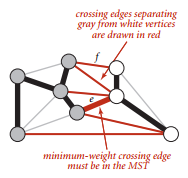
\includegraphics[scale=0.4]{./figures/mst2.png}

\smallskip

\tiny cut property
\end{center}
\end{itemize}
\end{frame}
\begin{frame}[fragile]
\begin{minipage}{200pt}
\begin{itemize}
\item greedy MST algorithm
\begin{itemize}
\item start with all edges colored gray

\item find cut with no black edges and color its minimum-weight edge black

\item repeat until $V - 1$ edges are colored black
\end{itemize}

\item the greedy algorithm computes the MST

\item Kruskal's and Prim's aogrithms that we will encounter later choose cuts and minimum-weight edges efficiently
\end{itemize}
\end{minipage}%
\begin{minipage}{100pt}
\begin{center}
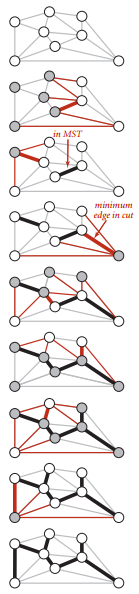
\includegraphics[scale=0.4]{./figures/mst3.png}

\smallskip

\tiny trace of greedy MST algorithm
\end{center}
\end{minipage}
\end{frame}

\section{Kruskal's Algorithm}
\begin{frame}[fragile]
\begin{minipage}{240pt}
\begin{itemize}
\item add edges to tree $T$ in ascending order of weight unless doing so would create a cycle
\begin{lstlisting}[language=Java]
public class KruskalMST {
    private double weight;  
    private LinkedQueue<Edge> mst;
    
    public KruskalMST(EdgeWeightedGraph G) {
        mst =  new LinkedQueue<Edge>();  
        HeapMinPQ<Edge> pq = new HeapMinPQ<Edge>();
        for (Edge e : G.edges()) { pq.insert(e); }
        WeightedQuickUnionUF uf = 
            new WeightedQuickUnionUF(G.V());
        while (!pq.isEmpty() && mst.size() < G.V() - 1) {
            Edge e = pq.delMin();
            int v = e.either();
            int w = e.other(v);
            if (!uf.connected(v, w)) { 
                uf.union(v, w); 
                mst.enqueue(e); 
                weight += e.weight();
            }
        }
    }

    public Iterable<Edge> edges() { return mst; }

    public double weight() { return weight; }
    ...
}
\end{lstlisting}

\item Kruskal's algorithm computes MST in time proportional to
$E \log E$ and extra space proportional to $V$ in the worst case
\end{itemize}
\end{minipage}%
\begin{minipage}{100pt}
\begin{center}
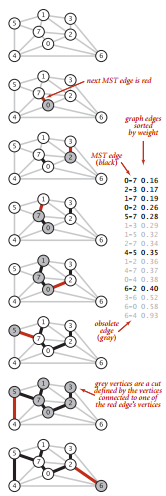
\includegraphics[scale=0.4]{./figures/mst4.png}

\smallskip

\tiny trace of Kruskal's algorithm
\end{center}
\end{minipage}
\end{frame}

\section{Prim's Algorithm}
\begin{frame}[fragile]
\begin{itemize}
\item approach
\begin{itemize}
\item start with vertex 0 and greedily grow tree $T$

\item add to $T$ the minimum-weight edge with exactly one endpoint in $T$

\item repeat until $V - 1$ edges have been added
\end{itemize}

\item challenge: find the minimum-weight edge with exactly one endpoint in $T$
\end{itemize}
\end{frame}

\begin{frame}[fragile]
\begin{itemize}
\item lazy approach: maintain a priority queue (PQ) of edges with (at least) one endpoint in $T$
\begin{itemize}
\item key = edge; priority = weight of edge

\item delete minimum to determine next edge $e$ = $v$-$w$ to add to $T$

\item disregard if both endpoints $v$ and $w$ are marked (both in $T$)

\item otherwise, let $w$ be the unmarked vertex (not in $T$)
\begin{itemize}
\item add to PQ any edge incident to $w$ (assuming other endpoint not in $T$)
\item add $e$ to $T$ and mark $w$
\end{itemize}
\end{itemize}

\begin{lstlisting}[language=Java]
public class LazyPrimMST {
    private double weight; 
    private LinkedQueue<Edge> mst; 
    private boolean[] marked; 
    private HeapMinPQ<Edge> pq; 

    public LazyPrimMST(EdgeWeightedGraph G) {
        mst = new LinkedQueue<Edge>();
        pq = new HeapMinPQ<Edge>();
        marked = new boolean[G.V()];
        for (int v = 0; v < G.V(); v++) {
            if (!marked[v]) prim(G, v);  
        }  
    }
    ...
}
\end{lstlisting}
\end{itemize}
\end{frame}

\begin{frame}[fragile]
\begin{minipage}{240pt}
\begin{itemize}
\item lazy approach (contd.) 
\begin{lstlisting}[language=Java]
public class LazyPrimMST {
    ...
    private void prim(EdgeWeightedGraph G, int s) {
        scan(G, s);
        while (!pq.isEmpty()) { 
            Edge e = pq.delMin(); 
            int v = e.either(), w = e.other(v);  
            if (marked[v] && marked[w]) { continue; }  
            mst.enqueue(e); 
            weight += e.weight();
            if (!marked[v]) { scan(G, v); }  
            if (!marked[w]) { scan(G, w); } 
        }
    }

    private void scan(EdgeWeightedGraph G, int v) {
        marked[v] = true;
        for (Edge e : G.adj(v)) {
            if (!marked[e.other(v)]) { pq.insert(e); }
        }
    }
    
    public Iterable<Edge> edges() { return mst; }

    public double weight() { return weight; }
    ...
}
\end{lstlisting}

\item lazy Prim's algorithm computes the MST in time proportional
to $E \log E$ and extra space proportional to $E$ in the worst case
\end{itemize}
\end{minipage}%
\begin{minipage}{90pt}
\begin{center}
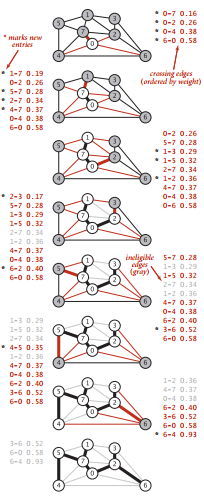
\includegraphics[scale=0.4]{./figures/mst5.png}

\smallskip

\tiny trace of Prims's algorithm (lazy approach)
\end{center}
\end{minipage}
\end{frame}

\begin{frame}[fragile]
\begin{itemize}
\item eager approach: maintain a PQ of vertices connected by an edge to $T$, where priority of vertex $v$ = weight of shortest edge connecting $v$ to $T$
\begin{itemize}
\item delete minimum vertex $v$ and add its associated edge $e$ = $v$-$w$ to $T$ 

\item update PQ by considering all edges $e$ = $v$-$x$ incident to $v$

\begin{itemize}
\item ignore if $x$ is already in $T$

\item add $x$ to PQ if not already on it

\item decrease priority of $x$ if $v$-$x$ becomes shortest edge connecting $x$ to $T$
\end{itemize}
\end{itemize}

\begin{lstlisting}[language=Java]
public class PrimMST {
    private Edge[] edgeTo; 
    private double[] distTo; 
    private boolean[] marked; 
    private IndexMinPQ<Double> pq;

    public PrimMST(EdgeWeightedGraph G) {
        edgeTo = new Edge[G.V()];
        distTo = new double[G.V()];
        marked = new boolean[G.V()];
        pq = new IndexMinPQ<Double>(G.V());
        for (int v = 0; v < G.V(); v++) { 
            distTo[v] = Double.POSITIVE_INFINITY;
        }
        for (int v = 0; v < G.V(); v++) {
            if (!marked[v]) { prim(G, v); }
        }
    }
    ...
}
\end{lstlisting}
\end{itemize}
\end{frame}

\begin{frame}[fragile]
\begin{itemize}
\item eager approach (contd.)

\begin{lstlisting}[language=Java]
public class PrimMST {
    ...
    private void prim(EdgeWeightedGraph G, int s) {
        distTo[s] = 0.0;
        pq.insert(s, distTo[s]);
        while (!pq.isEmpty()) {
            int v = pq.delMin();
            scan(G, v);
        }
    }

    private void scan(EdgeWeightedGraph G, int v) {
        marked[v] = true;
        for (Edge e : G.adj(v)) {
            int w = e.other(v);
            if (marked[w]) { continue; }
            if (e.weight() < distTo[w]) {
                distTo[w] = e.weight();
                edgeTo[w] = e;
                if (pq.contains(w)) { pq.decreaseKey(w, distTo[w]); }
                else                { pq.insert(w, distTo[w]); }
            }
        }
    }
    ...
}
\end{lstlisting}
\end{itemize}
\end{frame}
\begin{frame}[fragile]
\begin{minipage}{240pt}
\begin{itemize}
\item eager approach (contd.)

\begin{lstlisting}[language=Java]
public class PrimMST {
    ...
    public Iterable<Edge> edges() {
        LinkedQueue<Edge> mst = new LinkedQueue<Edge>();
        for (int v = 0; v < edgeTo.length; v++) {
            Edge e = edgeTo[v];
            if (e != null) { mst.enqueue(e); }
        }
        return mst;
    }

    public double weight() {
        double weight = 0.0;
        for (Edge e : edges()) { weight += e.weight(); }
        return weight;
    }
    ...
}
\end{lstlisting}

\item a binary heap based implementation of eager Prim's algorithm computes the MST in time proportional to $E \log V$ and extra space proportional to $V$ in the worst case
\end{itemize}
\end{minipage}%
\begin{minipage}{90pt}
\begin{center}
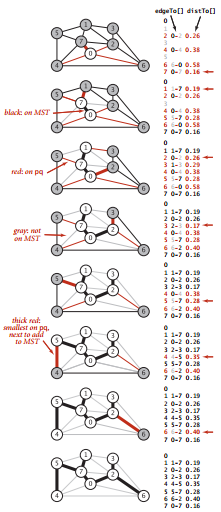
\includegraphics[scale=0.4]{./figures/mst6.png}

\smallskip

\tiny trace of Prims's algorithm (eager approach)
\end{center}
\end{minipage}
\end{frame}
\end{document}
